\documentclass[a4paper]{article}
\usepackage{listings}
\usepackage{color}
\usepackage[margin=1in]{geometry}
\usepackage{graphicx}

\definecolor{dkgreen}{rgb}{0,0.6,0}
\definecolor{gray}{rgb}{0.5,0.5,0.5}
\definecolor{mauve}{rgb}{0.58,0,0.82}

\lstset{frame=tb,
	language=C++,
	aboveskip=3mm,
	belowskip=3mm,
	showstringspaces=false,
	columns=flexible,
	basicstyle={\small\ttfamily},
	numbers=none,
	numberstyle=\tiny\color{gray},
	keywordstyle=\color{blue},
	commentstyle=\color{dkgreen},
	stringstyle=\color{mauve},
	breaklines=true,
	breakatwhitespace=true,
	tabsize=4
}

\begin{document}	
	\title{NOI 2016 Reference Sheet}
	\author{Compiled by Sun Yudong}
	\date{\today}
	\maketitle
	
	\begin{center}
		{\Huge \textbf{Don't Panic}}
	\end{center}
	
	\section{Sorts}
	\subsection{Merge Sort}
	\begin{lstlisting}
#include <iterator>
#include <algorithm> // for std::inplace_merge
#include <functional> // for std::less

template<typename RandomAccessIterator, typename Order>
void mergesort(RandomAccessIterator first, RandomAccessIterator last, Order order)
{
	if (last - first > 1)
	{
		RandomAccessIterator middle = first + (last - first) / 2;
		mergesort(first, middle, order);
		mergesort(middle, last, order);
		std::inplace_merge(first, middle, last, order);
	}
}

template<typename RandomAccessIterator>
void mergesort(RandomAccessIterator first, RandomAccessIterator last)
{
	mergesort(first, last, std::less<typename std::iterator_traits<RandomAccessIterator>::value_type>());
}
	\end{lstlisting}
	
	\subsection{Sort using Algorithm Package}
	Using arrays: 
	\begin{lstlisting}
// sort() Example using arrays.
// By Zereo 04/22/13
#include <iostream>
#include <algorithm>

using namespace std;

const int SIZE = 7;

int main()
{
	int intArray[SIZE] = {5, 3, 32, -1, 1, 104, 53};
	
	//Now we call the sort function
	sort(intArray, intArray + SIZE);
	
	//Alternatively in C++11
	sort(begin(intArray), end(intArray));
	
	cout << "Sorted Array looks like this." << endl;
	for (size_t i = 0; i != SIZE; ++i)
	cout << intArray[i] << " ";
	
	return 0;
}
	\end{lstlisting}
	
	And using vectors:
	\begin{lstlisting}
// Vector Sorting Example.
// By Zereo 04/22/13
#include <iostream>
#include <algorithm>
#include <vector>
#include <string>

using namespace std;

int main()
{
	// Warning this type of initialization requires a C++11 Compiler
	vector<int> intVec = {56, 32, -43, 23, 12, 93, 132, -154};
	vector<string> stringVec = {"John", "Bob", "Joe", "Zack", "Randy"};
	
	// Sorting the int vector
	sort(intVec.begin(), intVec.end());
	
	for (vector<int>::size_type i = 0; i != intVec.size(); ++i)
	cout << intVec[i] << " ";
	
	cout << endl;
	
	// Sorting the string vector
	sort(stringVec.begin(), stringVec.end());
	
	// Ranged Based loops. This requires a C++11 Compiler also
	// If you don't have a C++11 Compiler you can use a standard
	// for loop to print your vector.
	for (string &s : stringVec)
	cout << s << " ";
	
	return 0;
}
	\end{lstlisting}
	
	\section{Greatest Common Divisor}
	\begin{lstlisting}
unsigned int gcd(unsigned int u, unsigned int v)
{
	int shift;
	
	/* GCD(0,v) == v; GCD(u,0) == u, GCD(0,0) == 0 */
	if (u == 0) return v;
	if (v == 0) return u;
	
	/* Let shift := lg K, where K is the greatest power of 2 dividing both u and v. */
	for (shift = 0; ((u | v) & 1) == 0; ++shift) {
		u >>= 1;
		v >>= 1;
	}
	
	while ((u & 1) == 0) {
		u >>= 1;
	}
	
	/* From here on, u is always odd. */
	do {
		/* remove all factors of 2 in v -- they are not common */
		/*   note: v is not zero, so while will terminate */
		while ((v & 1) == 0)  /* Loop X */ {
			v >>= 1;
		}
		
		/* Now u and v are both odd. Swap if necessary so u <= v,
		then set v = v - u (which is even). For bignums, the
		swapping is just pointer movement, and the subtraction
		can be done in-place. */
		
		if (u > v) {
			unsigned int t = v; v = u; u = t;}	// Swap u and v.
			v = v - u;                       	// Here v >= u.
	} while (v != 0);
	
	/* restore common factors of 2 */
	return u << shift;
}
	\end{lstlisting}
	
	\section{deque}
	\begin{lstlisting}
deque();                   						//default constructor
deque<int> dq1;									//produces empty deque of ints

deque(const deque& d ); 						//copy constructor
deque<int> dq2(dq1);     						//creates a copy of dq1 in dq2
deque<int> dq2(dq1.begin(), dq1.end());
deque<int> dq2(dq1.rbegin(), dq1.rend());		//create a new deque, reversing dq1 by using reverse iterators

deque(size_type number, const T& value=T() );   //initialization construction
deque<double> dq3(10);     						//deque of doubles with 10 elements set to default (0.0)
deque<double> dq4(5, 8.1); 						//deque of doubles with 5 elements set to 8.1

deque(iterator start, iterator end );   		//interator constructor
double array1[]={0.0,1.0,2.0,3.0,4.0,5.0,6.0,7.0,8.0,9.0};
deque<double> dq5(array1,array1+4);      		//constructs deque with elements 0-3 from array1

/*----------*/

#include <stdexcept>	//required for defining and catching standard exceptions

deque<double> dq(5, 8.1);

for (int i=0; i<=5; ++i) {
	cout << "Element "<< i << " accessed with [] : "<< dq[i] << endl;
}

try {
	cout << "Element " << i << " accessed with at(i) :" << dq.at(i) << endl;
} catch (out_of_range&) {
	cout << "**out of range exception accessing element " << i << " with at() **" << endl;
}

/*---------*/

dq.at(2)=9.5				/* to change the element */
dq.size()					/* Size of deque */
(dq.empty())				/* Is deque empty? Return true if it is*/
dq.max_size()				/* Maximum size of deque */
dq.push_back(i)				/* Add elements to the back */
dq.push_front(i)			/* Add elements to the front */
dq.pop_front()				/* Remove first element */
dq.pop_back()				/* Remove last element */

/* display to screen */
for (int i=0; i<(signed)dq.size(); ++i) cout << dq.at(i);

/* insert array into deque */
int array[]= { 0, 1, 2, 3, 4 };
dq.insert(dq.begin()+2, array, array+5);

dq.insert(dq.begin()+4, 3, 0);		/* insert 3 copies of 0s */
dq.erase(dq.end()-2);				/* erase the next-to-last element */
	/* note: end() returns and iterator to the point just past the end of the queue. */
dq.erase(dq.begin(),dq.begin()+3);	/* erase the first three elements */

/* ----- */

//  declare two deques and intialize the second to contain 10 zeros
deque<int> dq1;
deque<int> dq2(10,0);

dq1.assign(10,5); 	/* assign 10 copies of the int 5 to deque 1 */
dq1.resize(15,10); 	/* resize deque 1, trailing elems truncated, new elems initialized to 10 */
dq1.swap(dq2);		/* swap contents of the deques */
dq1.clear();		/* clears and empties dq1, size will return 0 */

/* iterate through a deque */
for (deque<int>::iterator itr = dq.begin(); itr != dq.end(); ++itr)


	\end{lstlisting}
	
	\section{Vectors}
	\begin{lstlisting}
/* initializing a vector */
	vector<int> v { 34,23 };
	vector<int> v[1000005]; 
	
	vector<int> v(2);
	v = { 34,23 };
	
	vector<char> array;
	array.reserve(10) // If the vector already has room for the required number of elements, reserve() does nothing. In other words, reserve() will grow the allocated storage of the vector, if necessary, but will never shrink it.

/* using a vector */
v.push_back(1) 			//adds the element 1 to the end of the vector
v.capacity()			//vector capacity
v.size()				//actually how many elements there are
v.resize(6, 1);			//similar to deque

double a[] = {1, 2, 3, 4, 5};
mean(a, 5)
/* is equal to */
vector<double> a; //and you push the necessary elements
mean(&a[0], 5)

/* inserting array into vector */
double p[] = {1, 2, 3, 4, 5};
vector<double> a(p, p+5);

/* interating */
vector<double>::const_iterator i;
	for(i=a.begin(); i!=a.end(); ++i){
	std::cout<<(*i)<<std::endl;
}
	
	
	\end{lstlisting}
	
	\section{AARGHHHH}
	\begin{lstlisting}
/* always begin with the right bits */
#include <bits/stdc++.h>

/* reading/writing from/to standard input */
scanf("%d", &n);
printf("%d\n", n);

/* reading/writing to filestreams */
ifstream fin("file1.txt");
ofstream fout("output.txt");
!stream1.eof()					//check if end of file
	
/* initializing an array */
long long int x[1000] = {x1, x2, ....};

/* getting the whole line */
string name;
cin.getline (name, [chars], [delim]); /* or */
getline(cin, name);
	\end{lstlisting}
	
	\vspace{5mm}
	
	\begin{center}
		Here marks the end... Good luck! :D \\
		\vspace{5mm}
		{\Huge \textbf{Don't Panic}}
	\end{center}
	
	\begin{figure}[ht!]
		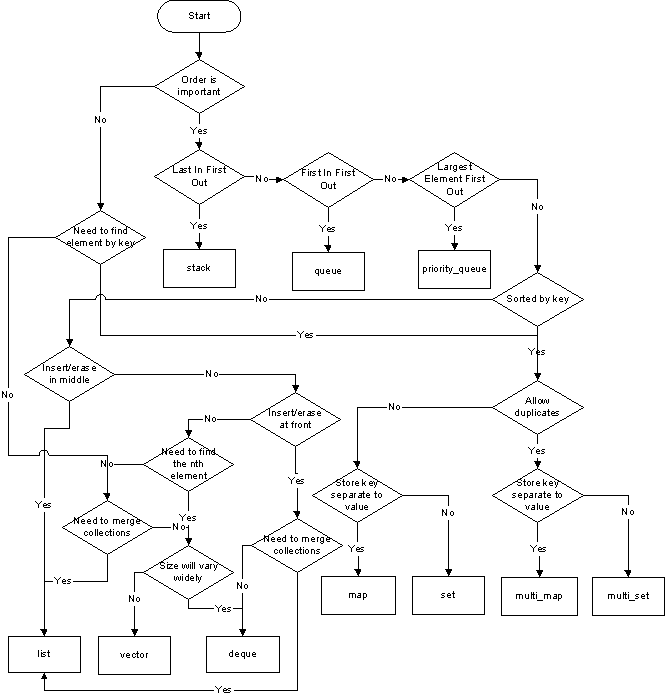
\includegraphics[width=\textwidth]{d5CDK.png}
	\end{figure}
	
\end{document}